\documentclass[11pt]{article}
\usepackage[margin=1in,letterpaper]{geometry}
\usepackage{amssymb,amsmath,amsthm,fancyhdr,supertabular,longtable,hhline}
\usepackage{colortbl}
\usepackage{import, multicol,boxedminipage}
\usepackage{graphicx}
\usepackage[colorlinks, hyperindex, plainpages=false, linkcolor=blue, urlcolor=blue, pdfpagelabels]{hyperref}
\usepackage[all]{hypcap}
\definecolor{ResultColor}{gray}{0.9}
\theoremstyle{definition}  % this prevents the text in definitions, theorems, and corollaries from being italicized
\newtheorem{defn}{\bf Definition}
\newtheorem{thm}{\bf Theorem}
\newtheorem{cor}[thm]{\bf Corollary}
\newtheorem{eqn}{\bf Equation}
\newtheorem{ex}{\bf Example}
\newtheorem{fig}{\bf Figure}
\setlength{\parindent}{0in}
\newcommand{\bbm}{\begin{boxedminipage}{6.41in}}
\newcommand{\ebm}{\end{boxedminipage}}
\usepackage{array}
\setlength{\extrarowheight}{2pt}
\allowdisplaybreaks[2]
\usepackage{cancel}
\usepackage{sectsty}
\usepackage{textcomp}
\usepackage{multirow}
\usepackage[sfdefault,lf]{carlito}
	%% The 'lf' option for lining figures
	%% The 'sfdefault' option to make the base font sans serif
	\usepackage[T1]{fontenc}
	\renewcommand*\oldstylenums[1]{\carlitoOsF #1}
\usepackage[nottoc]{tocbibind}
\allsectionsfont{\mdseries \scshape}
\makeatletter
\renewcommand\l@section{\@dottedtocline{1}{1.5em}{3em}}
\renewcommand\l@subsection{\@dottedtocline{2}{4.5em}{3.5em}}
\makeatother
\pagestyle{fancy}
\newcounter{HW}
\newcounter{HWindent}
%\makeindex

\title{Review \#2: Absolute Value Equations and Inequalities}
\author{Carl Stitz and Jeff Zeager\\
Edited by Sean Fitzpatrick}
\begin{document}
\maketitle


\renewcommand{\headrulewidth}{0pt}
\renewcommand{\headheight}{14pt}
\lhead[\fancyplain{}{\sc\thepage}]%
      {\fancyplain{}{\sc \nouppercase{\rightmark}}}
\rhead[\fancyplain{}{\sc \nouppercase{\leftmark}}]%
      {\fancyplain{}{\sc\thepage}}
\cfoot{}


In this section, we review some basic concepts involving the absolute value of a real number $x$.  There are a few different ways to define absolute value and in this section we choose the following definition.  (Absolute value will be revisited in much greater depth in the Math 1010 textbook, where we present what one can think of as the ``precise'' definition.)

\medskip

\colorbox{ResultColor}{\bbm

\begin{defn}\label{absvaldistdefn}{\bf Absolute Value as Distance:}  For every real number $x$, the \textbf{absolute value} of $x$, denoted $|x|$, is the distance between $x$ and $0$ on the number line.  More generally, if $x$ and $c$ are real numbers, $|x-c|$ is the distance between the numbers $x$ and $c$ on the number line.

\end{defn}

\ebm}

\medskip

For example, $|5| = 5$ and $|-5| = 5$, since each is $5$ units from $0$ on the number line:

\begin{center}

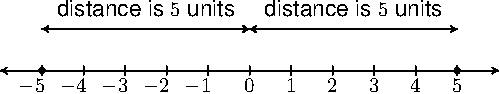
\includegraphics{AbsValEqIneq-1}

Graphically why $|-5| = 5$ and $|5| = 5$

\end{center}

Computationally, the absolute value `makes negative numbers positive',  though we need to be a little cautious with this description. While $|-7| = 7$, $|5-7| \neq 5+7$.  The absolute value acts as a grouping symbol, so $|5-7| = |-2| = 2$, which makes sense since $5$ and $7$ are two units away from each other on the number line:

\begin{center}

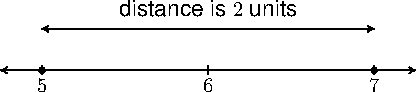
\includegraphics{AbsValEqIneq-2}

Graphical illustration of why $|5-7| = 2$

\end{center}

We list some of the operational properties of absolute value below.

\medskip

\colorbox{ResultColor}{\bbm
\begin{thm}  \textbf{Properties of Absolute Value:} Let $a$, $b$ and $x$ be real numbers and let $n$ be an integer. Then \label{absolutevalueprops} 

\begin{itemize}

\item {\bf Product Rule:} $|ab|= |a||b|$ 

\item {\bf Power Rule:} $\left| a^{n} \right| = |a|^{n}$ whenever $a^{n}$ is defined 

\item {\bf Quotient Rule:} $\left| \dfrac{a}{b} \right| = \dfrac{|a|}{|b|}$, provided $b \neq 0$ 

\end{itemize}

\end{thm}

\ebm}

\medskip

The proof of Theorem \ref{absolutevalueprops} is difficult, but not impossible, using the distance definition of absolute value or even the `it makes negatives positive' notion.  It is, however, much easier if one uses the ``precise'' definition given in the textbook, so we will omit the proof for now. For now, let's focus on how to solve basic equations and inequalities involving the absolute value.

\section{Absolute Value Equations}
\label{basicabsvaleqns}

Thinking of absolute value in terms of distance gives us a geometric way to interpret equations.  For example, to solve $|x| = 3$, we are looking for all real numbers $x$ whose distance from $0$ is $3$ units.  If we move three units to the right of $0$, we end up at $x = 3$.  If we move three units to the left, we end up at $x = -3$.  Thus the solutions to  $|x| = 3$ are $x = \pm 3$.  


\begin{center}

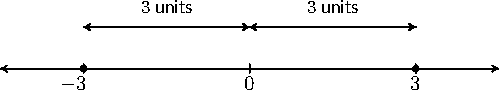
\includegraphics{AbsValEqIneq-3}

The solutions to  $|x| = 3$ are $x = \pm 3$.  

\end{center}



Thinking this way gives us the following.

\medskip

\colorbox{ResultColor}{\bbm

\begin{thm} \textbf{Absolute Value Equations: }\label{absvalequality}  Suppose $x$, $y$ and $c$ are real numbers.

\begin{itemize}

\item  $|x| = 0$ if and only if $x = 0$.

\item  For $c > 0$, $|x| = c$ if and only if $x = c$ or $x = -c$.

\item  For $c < 0$, $|x| = c$ has no solution.

\item  $|x| = |y|$ if and only if $x = y$ or $x = -y$. 

(That is,  if two numbers have the same absolute values, they are either the same number or exact opposites.) 

\end{itemize}

\end{thm}

\ebm}

\medskip

Theorem \ref{absvalequality} is our main tool in solving equations involving the absolute value, since it allows us a way to rewrite such equations as compound linear equations.

\medskip

\phantomsection
\label{strategyforsolvingabseqns}

\colorbox{ResultColor}{\bbm

\centerline{\textbf{Strategy for Solving Equations Involving Absolute Value}}

\vspace{0.05in}

In order to solve an equation involving the absolute value of a quantity $|X|$:

\begin{enumerate}

\item  Isolate the absolute value on one side of the equation so it has the form $|X| = c$.

\item  Apply Theorem \ref{absvalequality}.

\end{enumerate}

\ebm}

\medskip

The techniques we use to `isolate the absolute value' are precisely those we used in the handout on solving linear equations and inequalities (Review \#1) to isolate the variable when solving linear equations.  Time for some practice.

\begin{ex} \label{absvalueeqnex}  Solve each of the following equations.

\begin{multicols}{3}
\begin{enumerate}

\item  $|3x-1| = 6$\vphantom{ $\dfrac{3 - |y+5|}{2} = 1$}
\item  $\dfrac{3 - |y+5|}{2} = 1$
\item  $3|2t+1| - \sqrt{5} = 0$\vphantom{ $\dfrac{3 - |y+5|}{2} = 1$}

\setcounter{HW}{\value{enumi}}
\end{enumerate}
\end{multicols}

\begin{multicols}{3}
\begin{enumerate}
\setcounter{enumi}{\value{HW}}

\item  $4 - |5w+3| = 5$\vphantom{$\left|3 - x \sqrt[3]{12}\right| = |4x+1|$}

\item  $\left|3 - x \sqrt[3]{12}\right| = |4x+1|$\vphantom{$\left|3 - x \sqrt[3]{12}\right| = |4x+1|$}

\item  $|t-1| - 3|t+1| = 0$\vphantom{$\left|3 - x \sqrt[3]{12}\right| = |4x+1|$}


\end{enumerate}
\end{multicols}

{\bf Solution.} 

\begin{enumerate}

\item  The equation  $|3x-1| = 6$ is of already in the form $|X| = c$, so we know  $3x-1=6$ or $3x-1 = -6$.  Solving the former gives us at $x = \frac{7}{3}$ and solving the latter yields $x = -\frac{5}{3}$.  We may check both of these solutions by substituting them into the original equation and showing that the arithmetic works out.

\item  We begin solving  $\frac{3 - |y+5|}{2} = 1$ by isolating the absolute value to put it in the form $|X| = c$.\[ \begin{array}{rclr}
\dfrac{3 - |y+5|}{2} & = & 1 &  \\
3 - |y+5| & = & 2 & \text{Multiply by $2$}\\
-|y+5| & = & -1 & \text{Subtract $3$} \\
|y+5| & = & 1 & \text{Divide by $-1$}  \\ 

\end{array} \] At this point, we have $y+5 = 1$ or $y+5 = -1$, so our solutions are $y = -4$ or $y = -6$.  We leave it to the reader to check both answers in the original equation.

\item As in the previous example, we first isolate the absolute value.  Don't let the $\sqrt{5}$ throw you off - it's just another real number, so we treat it as such:\[ \begin{array}{rclr}

 3|2t+1| - \sqrt{5} & = & 0 & \\
 3|2t+1|  & = &  \sqrt{5} & \text{Add $\sqrt{5}$} \\
 |2t + 1| & = & \dfrac{\sqrt{5}}{3} & \text{Divide by $3$}\\
\end{array} \] From here, we have that $2t+1 = \frac{\sqrt{5}}{3}$ or $2t+1 = -\frac{\sqrt{5}}{3}$. The first equation gives $t = \frac{\sqrt{5}-3}{6}$ while the second gives $t = \frac{-\sqrt{5}-3}{6}$ thus we list our answers as $t = \frac{-3 \pm \sqrt{5}}{6}$.   The reader should enjoy the challenge of substituting both answers into the original equation and following through the arithmetic to see that both answers work.

\item  Upon isolating the absolute value in the equation $4 - |5w+3| = 5$, we get $|5w+3| = -1$.  At this point, we know there cannot be any real solution.  By definition, the absolute value is a \textit{distance}, and as such is never negative.  We write `no solution' and carry on.

\item Our next equation already has the absolute value expressions (plural) isolated, so we work from the principle that if $|x| = |y|$, then $x = y$ or $x = -y$. Thus from $\left|3 - x \sqrt[3]{12}\right| = |4x+1|$ we get two equations to solve:  \[ 3 - x \sqrt[3]{12} = 4x+1, \qquad \text{and} \qquad 3 - x \sqrt[3]{12} = -(4x+1) \] Notice that the right side of the second equation is $-(4x+1)$ and not simply $-4x+1$.  Remember, the expression $4x+1$ represents a single real number so in order to negate it we need to negate the \textit{entire} expression $-(4x+1)$. Moving along, when solving $3 - x \sqrt[3]{12} = 4x+1$, we obtain $x = \frac{2}{4 + \sqrt[3]{12}}$ and the solution to $3 - x \sqrt[3]{12} = -(4x+1)$ is $x = \frac{4}{\sqrt[3]{12}-4}$.  As usual, the reader is invited to check these answers by substituting them into the original equation.

\item We start by isolating one of the absolute value expressions:  $|t-1| - 3|t+1| = 0$ gives $|t-1| = 3|t+1|$.  While this \textit{resembles} the form $|x| = |y|$, the coefficient $3$ in $3|t+1|$ prevents it from being an exact match.  Not to worry - since $3$ is positive, $3 = |3|$ so \[3|t+1| = |3| |t+1| = |3(t+1)| = |3t+3|.\]  Hence, our equation becomes $|t-1| = |3t+3|$ which results in the two equations:  $t-1 = 3t+3$ and $t-1 = -(3t+3)$.  The first equation gives $t = -2$ and the second gives $t = -\frac{1}{2}$.  The reader is encouraged to check both answers in the original equation. \qed

\end{enumerate}

\end{ex}


\section{Absolute Value Inequalities}
\label{basicabsvalineq}

We now turn our attention to solving some basic inequalities involving the absolute value.  Suppose we wished to solve $|x| < 3$.  Geometrically, we are looking for all of the real numbers whose distance from $0$ is \textit{less} than $3$ units.  We get $-3 < x < 3$, or in interval notation, $(-3,3)$.  Suppose we are asked to solve $|x| > 3$ instead.  Now we want the distance between $x$ and $0$ to be \textit{greater} than $3$ units.  Moving in the positive direction, this means $x > 3$.  In the negative direction, this puts $x < -3$.  Our solutions would then satisfy $x < -3$ \textit{or} $x > 3$.  In interval notation, we express this as $(-\infty, -3) \cup (3, \infty)$.  


\begin{center}

\begin{tabular}{cc}

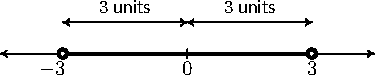
\includegraphics{AbsValEqIneq-4}

& 

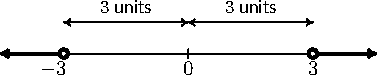
\includegraphics{AbsValEqIneq-5}

\\




The solution to  $|x| < 3$ is $(-3,3)$ &   The solution to  $|x| > 3$ is $(-\infty, -3) \cup (3, \infty)$ \\

\end{tabular}

\end{center}

Generalizing this notion, we get the following:

\medskip

\colorbox{ResultColor}{\bbm
\begin{thm}  \label{absolutevalueineq} \textbf{Inequalities Involving Absolute Value:}  Let $c$ be a real number.  

\begin{itemize}

\item   If $c> 0$, $|x| < c$ is equivalent to $-c<x<c$.

\item  If $c \leq 0$, $|x| < c$ has no solution.

\item  If $c > 0$, $|x| > c$ is equivalent to $x < -c$ or $x > c$.

\item If $c \leq 0$, $|x| > c$ is true for all real numbers.

\end{itemize}

\end{thm}
\ebm}

\medskip

If the inequality we're faced with involves `$\leq$' or `$\geq$,' we can combine the results of Theorem \ref{absolutevalueineq}  with Theorem \ref{absvalequality} as needed. 

\medskip

\phantomsection
\label{strategyforsolvingabsineq}

\colorbox{ResultColor}{\bbm

\centerline{\textbf{Strategy for Solving Inequalities Involving  Absolute Value}}

\vspace{0.05in}

In order to solve an inequality involving the absolute value of a quantity $|X|$:

\begin{enumerate}

\item  Isolate the absolute value on one side of the inequality.

\item  Apply Theorem \ref{absolutevalueineq}.

\end{enumerate}

\ebm}

\medskip

\begin{ex}  Solve the following inequalities.

\begin{multicols}{2}
\begin{enumerate}

\item  $\left|x-\sqrt[4]{5} \right| > 1$\vphantom{$\dfrac{4 - 2|2x+1|}{4} > -\sqrt{3}$}

\item  $\dfrac{4 - 2|2x+1|}{4} \geq -\sqrt{3}$

\setcounter{HW}{\value{enumi}}
\end{enumerate}
\end{multicols}

\begin{multicols}{2}
\begin{enumerate}
\setcounter{enumi}{\value{HW}}

\item  $|2x - 1| \leq 3|4 - 8x| - 10$

\item  $|2x - 1| \leq 3|4 - 8x| + 10$

\setcounter{HW}{\value{enumi}}
\end{enumerate}
\end{multicols}

\begin{multicols}{2}
\begin{enumerate}
\setcounter{enumi}{\value{HW}}



\item  $2 < |x-1| \leq 5$\vphantom{$\left|\sqrt{10} x - 5 \right| + \left|\sqrt{10} - 5x \right| \leq 0$
}

\item  $|10 x - 5| +|10 - 5x| \leq 0$


\setcounter{HW}{\value{enumi}}
\end{enumerate}
\end{multicols}

{\bf Solution.}  

\begin{enumerate}

\item  From Theorem \ref{absolutevalueineq}, $\left|x-\sqrt[4]{5} \right| > 1$ is equivalent to $x-\sqrt[4]{5} < -1$ or $x-\sqrt[4]{5} > 1$. Solving this compound inequality, we get $x < -1 + \sqrt[4]{5}$ or $x > 1 + \sqrt[4]{5}$.  Our answer, in interval notation, is:  $\left(-\infty,-1 + \sqrt[4]{5} \right) \cup \left(1 + \sqrt[4]{5},\infty \right)$.  As with linear inequalities, we can partially check our answer by selecting values of $x$ both inside and outside the solution intervals to see which values of $x$ satisfy the original inequality and which do not.

\item  Our first step in solving $\frac{4 - 2|2x+1|}{4} \geq -\sqrt{3}$ is to isolate the absolute value. \[ \begin{array}{rclr}
\dfrac{4 - 2|2x+1|}{4} & \geq & -\sqrt{3} & \\ [5pt]

4 - 2|2x+1| & \geq & -4\sqrt{3} & \text{Multiply by $4$} \\
- 2|2x+1| & \geq & -4-4\sqrt{3} & \text{Subtract $4$} \\
|2x+1| & \leq & \dfrac{-4-4\sqrt{3}}{-2} & \text{Divide by $-2$,  reverse the inequality} \\ [8pt]
|2x+1| & \leq & 2 + 2\sqrt{3} & \text{Reduce} \\ 

\end{array}\] Since we're dealing with `$\leq$' instead of just `$<$,' we can combine Theorems \ref{absolutevalueineq} and  \ref{absvalequality} to rewrite this last inequality as:\footnote{Note the use of parentheses: $-(2+2\sqrt{3})$ as opposed to $-2 + 2\sqrt{3}$.}   $-(2 + 2\sqrt{3}) \leq 2x+1 \leq 2+2\sqrt{3}$. Subtracting the `$1$' across both inequalities gives $-3-2\sqrt{3} \leq 2x \leq 1 + 2\sqrt{3}$, which reduces to $\frac{-3-2\sqrt{3}}{2} \leq x \leq \frac{1+2\sqrt{3}}{2}$.  In interval notation this reads as  $\left[\frac{-3-2\sqrt{3}}{2}, \frac{1+2\sqrt{3}}{2}\right]$.

\item  There are two absolute values in $|2x - 1| \leq 3|4 - 8x| - 10$, so it is unclear how we are to proceed.  However, before jumping in and trying to apply (or misapply) Theorem \ref{absolutevalueineq}, we note that $|4 - 8x| = |(-4)(2x-1)|$.   Using this, we get:\[ \begin{array}{rclr}

|2x - 1| & \leq & 3|4 - 8x| - 10 & \\

|2x - 1| & \leq & 3|(-4)(2x-1)| - 10 & \text{Factor}\\

|2x - 1| & \leq & 3|-4||2x-1| - 10 & \text{Product Rule}\\

|2x - 1| & \leq & 12|2x-1| - 10 & \\

-11|2x - 1| & \leq & - 10 & \text{Subtract $12|2x-1|$} \\

|2x - 1| & \geq  & \dfrac{10}{11} & \text{Divide by $-11$ and reduce} \\

\end{array}\] At this point, we invoke Theorems \ref{absvalequality} and \ref{absolutevalueineq} and write the equivalent compound inequality:  $2x - 1 \leq -\frac{10}{11}$ \textit{or} $2x-1 \geq \frac{10}{11}$.  We get $x \leq \frac{1}{22}$ \textit{or} $x \geq \frac{21}{22}$, which, in interval notation reads $\left(-\infty, \frac{1}{22}\right] \cup \left[\frac{21}{22}, \infty\right)$.

\item  The inequality  $|2x - 1| \leq 3|4 - 8x| + 10$ differs from the previous example in exactly one respect: on the right side of the inequality, we have `$+10$' instead of `$-10$.' The steps to isolate the absolute value here are identical to those in the previous example, but instead of obtaining $|2x - 1| \geq  \frac{10}{11}$ as before, we obtain $|2x - 1| \geq  -\frac{10}{11}$.  This latter inequality is \textit{always} true. (Absolute value is, by definition, a distance and hence always $0$ or greater.)  Thus our solution to this inequality is all real numbers, $(-\infty, \infty)$.


\item  To solve  $2 < |x-1| \leq 5$, we rewrite it as the compound inequality: $2 < |x-1|$ \textit{and} $|x-1| \leq 5$.   The first inequality, $2 < |x-1|$, can be re-written as $|x-1|>2$ so it is equivalent to  $x-1 < -2$ \textit{or} $x-1 > 2$.  Thus the solution to $2 < |x-1|$ is $x<-1$ or $x>3$, which in interval notation is  $(-\infty, -1) \cup (3, \infty)$.  For $|x-1| \leq 5$, we combine the results of Theorems \ref{absvalequality} and \ref{absolutevalueineq} to get $-5 \leq x-1 \leq 5$ so that $-4 \leq x \leq 6$, or $[-4,6]$.  Our solution to   $2 < |x-1| \leq 5$ is comprised of values of $x$ which satisfy both parts of the inequality, so we intersect $(-\infty, -1) \cup (3, \infty)$ with $[-4,6]$ to get our final answer $[-4,-1) \cup (3,6]$. 

\item Our first hope when encountering $|10 x - 5| + |10 - 5x| \leq 0$ is that we can somehow combine the two absolute value quantities as we'd done in earlier examples.  We leave it to the reader to show, however, that no matter what we try to factor out of the absolute value quantities, what remains inside the absolute values will always be different.  At this point, we take a step back and look at the equation in a more general way:  we are adding two absolute values together and wanting the result to be less than or equal to $0$.  Since the absolute value of anything is always $0$ or greater, there are no solutions to:  $|10x - 5| + |10 - 5x| < 0$.  Is it possible that $|10x - 5| + |10 - 5x| = 0$?  Only if there is an $x$ where $|10x-5| = 0$ and $|10-5x| = 0$ \textit{at the same time}.\footnote{Do you see why?}  The first equation holds only when $x = \frac{1}{2}$, while the second holds only when $x = 2$.  Alas, we have no solution.\footnote{Not for lack of trying, however!}   \qed

\end{enumerate}

\end{ex}

We close this section with an example of how the properties in Theorem \ref{absolutevalueprops} are used in Calculus.  Here, `$\varepsilon$' is the Greek letter `epsilon' and it represents a positive real number.  Those of you who will be taking Calculus in the future should become \emph{very} familiar with this type of algebraic manipulation.\[ \begin{array}{rclr}

\left| \dfrac{8-4x}{3} \right| & < & \varepsilon & \\ [12pt]

\dfrac{|8 - 4x|}{|3|} & < & \varepsilon & \text{Quotient Rule}\\ [12pt]

\dfrac{|-4(x-2)|}{3} & < & \varepsilon & \text{Factor} \\ [12pt]

\dfrac{|-4| |x-2|}{3} & < & \varepsilon & \text{Product Rule} \\ [12pt]

\dfrac{4 |x-2|}{3} & < & \varepsilon & \\ [12pt]

\dfrac{3}{4} \cdot \dfrac{4 |x-2|}{3} & < & \dfrac{3}{4} \cdot \varepsilon & \text{Multiply by $\dfrac{3}{4}$} \\ [12pt]

|x -2 | & < & \dfrac{3}{4} \varepsilon & \\  \end{array}\]

\newpage

\section{Exercises}

In Exercises \ref{solveabsvalequfirst} - \ref{solveabsvalequlast}, solve the equation.


\begin{multicols}{3}
\begin{enumerate}

\item  $|x| = 6$ \label{solveabsvalequfirst} 
\item $|3t-1| = 10$
\item $|4-w| = 7$

\setcounter{HW}{\value{enumi}}
\end{enumerate}
\end{multicols}

\begin{multicols}{3}
\begin{enumerate}
\setcounter{enumi}{\value{HW}}

\item  $4 - |y| = 3$
\item $2|5m+1| - 3 = 0$
\item $|7x-1| + 2 = 0$

\setcounter{HW}{\value{enumi}}
\end{enumerate}
\end{multicols}

\begin{multicols}{3}
\begin{enumerate}
\setcounter{enumi}{\value{HW}}

\item $\dfrac{5 - |x|}{2} = 1$ \vphantom{$\dfrac{|2x+1| - 3}{4} = \dfrac{1}{2} - |2x+1|$}
\item $\dfrac{2}{3} |5-2w| - \dfrac{1}{2} = 5$ \vphantom{$\dfrac{|2x+1| - 3}{4} = \dfrac{1}{2} - |2x+1|$}
\item $|3t - \sqrt{2}| + 4 = 6$ 
\setcounter{HW}{\value{enumi}}
\end{enumerate}
\end{multicols}


\begin{multicols}{3}
\begin{enumerate}
\setcounter{enumi}{\value{HW}}

\item $\dfrac{|2v+1| - 3}{4} = \dfrac{1}{2} - |2v+1|$
\item $|2x+1| = \dfrac{|2x+1| - 3}{2}$\vphantom{$\dfrac{|2v+1| - 3}{4} = \dfrac{1}{2} - |2v+1|$}
\item $\dfrac{|3-2y|+ 4}{2} = 2 - |3-2y|$\vphantom{$\dfrac{|2v+1| - 3}{4} = \dfrac{1}{2} - |2v+1|$}

\setcounter{HW}{\value{enumi}}
\end{enumerate}
\end{multicols}



\begin{multicols}{3}
\begin{enumerate}
\setcounter{enumi}{\value{HW}}

\item $|3t - 2| = |2t + 7|$  
\item $|3x+1| = |4x|$
\item $|1-\sqrt{2} y| = |y+1|$

\setcounter{HW}{\value{enumi}}
\end{enumerate}
\end{multicols}


\begin{multicols}{3}
\begin{enumerate}
\setcounter{enumi}{\value{HW}}

\item  $|4-x| - |x+2| = 0$
\item $|2-5z| = 5 |z+1|$
\item $\sqrt{3}|w-1| = 2|w+1|$ \label{solveabsvalequlast}


\setcounter{HW}{\value{enumi}}
\end{enumerate}
\end{multicols}


In Exercises \ref{solveinequabsquadfirst} - \ref{solveinequabsquadlast}, solve the inequality.  Write your answer using interval notation. 

\begin{multicols}{3}
\begin{enumerate}
\setcounter{enumi}{\value{HW}}
\item $|3x - 5| \leq 4$ \label{solveinequabsquadfirst}
\item $|7t + 2| > 10$
\item $|2w+1| - 5 < 0$   
\setcounter{HW}{\value{enumi}}
\end{enumerate}
\end{multicols}

\begin{multicols}{3}
\begin{enumerate}
\setcounter{enumi}{\value{HW}}


\item $|2-y| - 4 \geq -3$
\item $|3z+5| + 2 < 1$   
\item $2|7-v| +4 > 1$

\setcounter{HW}{\value{enumi}}
\end{enumerate}
\end{multicols}

\begin{multicols}{3}
\begin{enumerate}
\setcounter{enumi}{\value{HW}}


\item $3 - |x+\sqrt{5}| < -3$
\item $|5t| \leq |t|+3$   
\item $|w-3| < |3-w|$

\setcounter{HW}{\value{enumi}}
\end{enumerate}
\end{multicols}

\begin{multicols}{3}
\begin{enumerate}
\setcounter{enumi}{\value{HW}}

\item  $2 \leq |4-y| < 7$ 
\item $1 < |2w - 9| \leq 3$ 
\item  $3 > 2|\sqrt{3} - x| > 1$ \label{solveinequabsquadlast}
\setcounter{HW}{\value{enumi}}
\end{enumerate}
\end{multicols}

\begin{enumerate}
\setcounter{enumi}{\value{HW}}
\item  With help from your classmates, solve:
\begin{enumerate}
\item  $|5 - |2x-3|| = 4$
\item   $|5 - |2x-3|| < 4$
 
\end{enumerate}

\end{enumerate}


\newpage

\section{Answers}

\begin{multicols}{3}
\begin{enumerate}

\item  $x = -6$ or $x=6$ \vphantom{$t = -3$ or $t= \dfrac{11}{3}$}

\item $t = -3$ or $t= \dfrac{11}{3}$

\item $w = -3$ or $w= 11$ \vphantom{$t = -3$ or $t= \dfrac{11}{3}$}

\setcounter{HW}{\value{enumi}}
\end{enumerate}
\end{multicols}

\begin{multicols}{3}
\begin{enumerate}
\setcounter{enumi}{\value{HW}}

\item  $y = -1$ or $y= 1$\vphantom{$m=-\dfrac{1}{2}$ or $m= \dfrac{1}{10}$}

\item $m=-\dfrac{1}{2}$ or $m= \dfrac{1}{10}$

\item No solution\vphantom{$m=-\dfrac{1}{2}$ or $m= \dfrac{1}{10}$}

\setcounter{HW}{\value{enumi}}
\end{enumerate}
\end{multicols}

\begin{multicols}{3}
\begin{enumerate}
\setcounter{enumi}{\value{HW}}

\item  $x=-3$ or $x= 3$\vphantom{$t = \dfrac{\sqrt{2} \pm 2}{3}$}

\item $w = -\dfrac{13}{8}$ or $w= \dfrac{53}{8}$\vphantom{$t = \dfrac{\sqrt{2} \pm 2}{3}$}

\item $t = \dfrac{\sqrt{2} \pm 2}{3}$


\setcounter{HW}{\value{enumi}}
\end{enumerate}
\end{multicols}


\begin{multicols}{3}
\begin{enumerate}
\setcounter{enumi}{\value{HW}}

\item $v = -1$ or $v = 0$ \vphantom{$y = \dfrac{3}{2}$}

\item  No solution\vphantom{$y = \dfrac{3}{2}$}

\item  $y = \dfrac{3}{2}$

\setcounter{HW}{\value{enumi}}
\end{enumerate}
\end{multicols}



\begin{multicols}{3} 
\begin{enumerate}
\setcounter{enumi}{\value{HW}}

\item $t = -1$ or $t = 9$\vphantom{$x = -\dfrac{1}{7}$ or $x = 1$}

\item $x = -\dfrac{1}{7}$ or $x = 1$

\item $y = 0$ or $y = \dfrac{2}{\sqrt{2} - 1}$ 

\setcounter{HW}{\value{enumi}}
\end{enumerate}
\end{multicols}

\begin{multicols}{3} 
\begin{enumerate}
\setcounter{enumi}{\value{HW}}

\item $x=1$\vphantom{$w = \dfrac{\sqrt{3} \pm 2}{\sqrt{3} \mp 2}$}

\item $z = -\dfrac{3}{10}$\vphantom{$w = \dfrac{\sqrt{3} \pm 2}{\sqrt{3} \mp 2}$}

\item $w = \dfrac{\sqrt{3} \pm 2}{\sqrt{3} \mp 2}$ 

See footnote\footnote{That is, $w = \dfrac{\sqrt{3} + 2}{\sqrt{3} - 2}$ or $w = \dfrac{\sqrt{3} - 2}{\sqrt{3} + 2}$} 

\setcounter{HW}{\value{enumi}}
\end{enumerate}
\end{multicols}

\begin{multicols}{3}
\begin{enumerate}
\setcounter{enumi}{\value{HW}}

\item $\left[\dfrac{1}{3}, 3\right]$\vphantom{$\left(-\infty, -\dfrac{12}{7} \right) \cup \left(\dfrac{8}{7}, \infty\right)$}  
\item $\left(-\infty, -\dfrac{12}{7} \right) \cup \left(\dfrac{8}{7}, \infty\right)$
\item $(-3,2)$\vphantom{$\left(-\infty, -\dfrac{12}{7} \right) \cup \left(\dfrac{8}{7}, \infty\right)$}  
\setcounter{HW}{\value{enumi}}
\end{enumerate}
\end{multicols}

\begin{multicols}{3}
\begin{enumerate}
\setcounter{enumi}{\value{HW}}

 
\item $(-\infty,1] \cup [3,\infty)$
\item No solution  
\item $(-\infty, \infty)$

\setcounter{HW}{\value{enumi}}
\end{enumerate}
\end{multicols}

\begin{multicols}{2}
\begin{enumerate}
\setcounter{enumi}{\value{HW}}


\item $(-\infty, -6-\sqrt{5}) \cup (6-\sqrt{5}, \infty)$ \vphantom{$\left[ -\dfrac{3}{4}, \dfrac{3}{4}\right]$}
\item $\left[ -\dfrac{3}{4}, \dfrac{3}{4}\right]$   


\setcounter{HW}{\value{enumi}}
\end{enumerate}
\end{multicols}

\begin{multicols}{3}
\begin{enumerate}
\setcounter{enumi}{\value{HW}}

\item No solution 
\item $(-3,2] \cup [6,11)$

\item $[3, 4) \cup (5, 6]$

\setcounter{HW}{\value{enumi}}
\end{enumerate}
\end{multicols}

\begin{enumerate}
\setcounter{enumi}{\value{HW}}

\item $\left(\dfrac{2 \sqrt{3} - 3}{2},  \dfrac{2 \sqrt{3} - 1}{2}   \right) \cup \left(\dfrac{2 \sqrt{3} +1}{2},  \dfrac{2 \sqrt{3} +3}{2}   \right)$

\item  \begin{enumerate} \item $x = -3$, or $x = 1$, or $x = 2$, or $x = 6$

\item $(-3,1) \cup (2,6)$

\end{enumerate}

\setcounter{HW}{\value{enumi}}
\end{enumerate}


\end{document}